\section{Zooming into langages with unexpected behevior}\label{zoom}
It would not possible to present the results for all the languages which contradict a universal MAL hypothesis. An online website will all the results will be proposed with the final version. Here we will present some remarkable cases of Anti MAL languages, as well as some cases of languages with inconsistnent behavior in the pre- and/por postverbal domains. 

One interesting example of an Anti MAL language is the OldEast Slavic, which not only has an Anti MAL effect (that is, the mean length of the constituents increase with the number of constituents), but on top of that the Anti MAL effect increases with the number of constituents (Figure \ref{fig:OldEastSlavic})

\begin{figure}[!ht]
\begin{center}
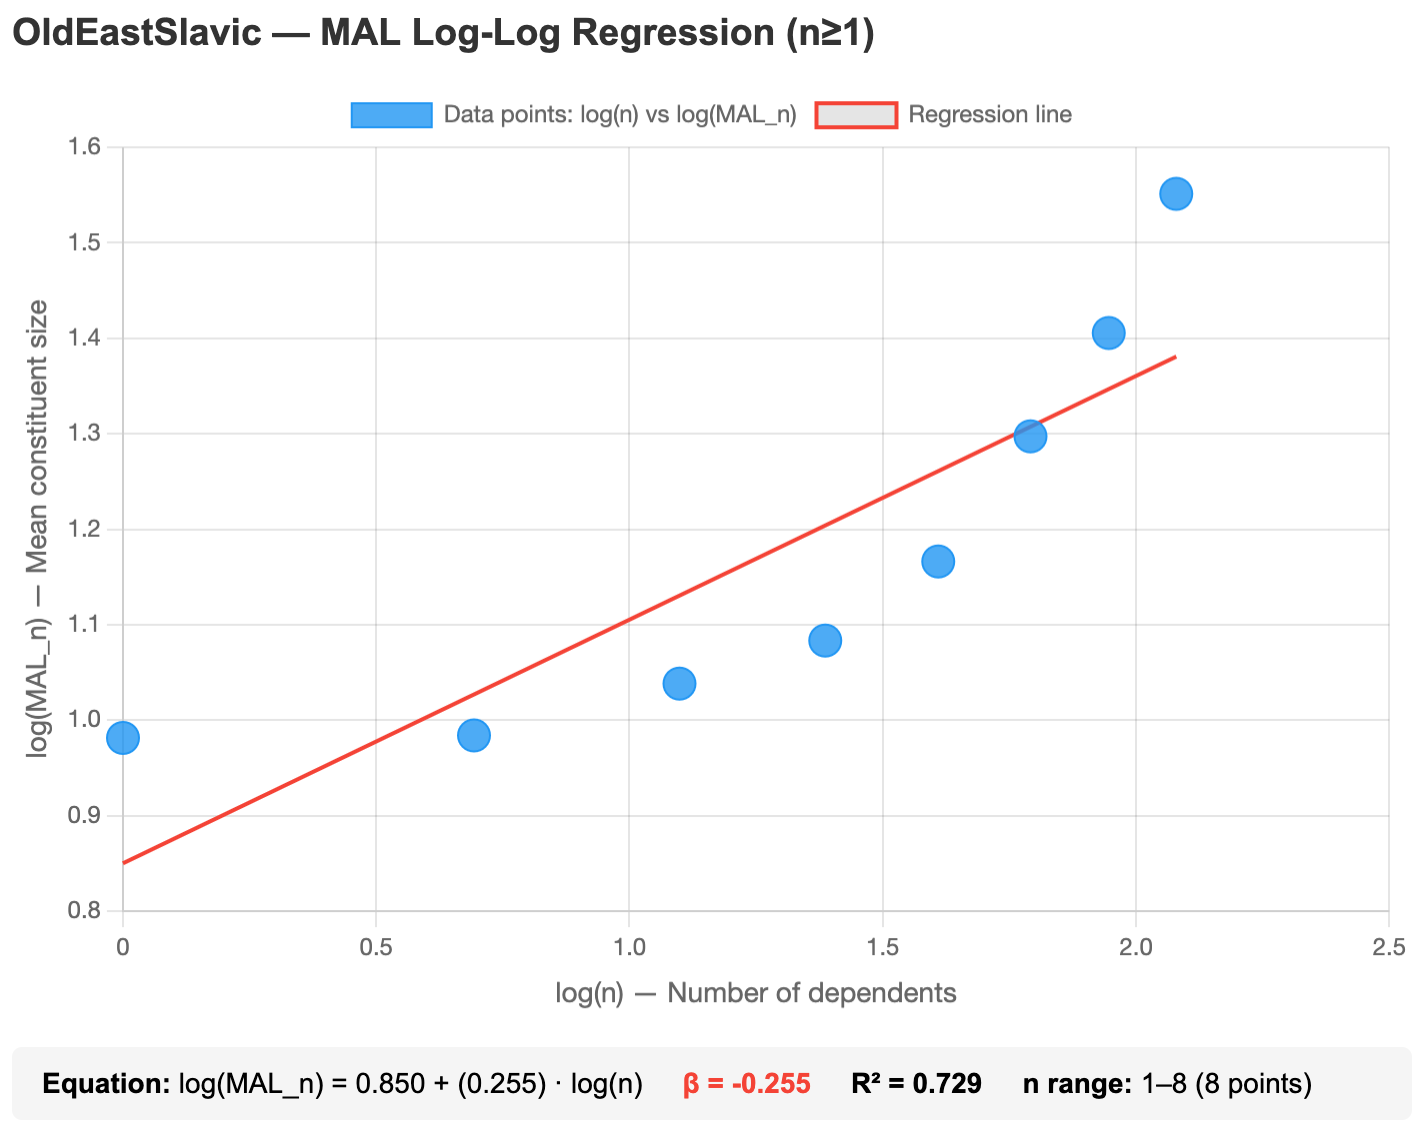
\includegraphics[width=\columnwidth]{latex/OldEastSlavic.png}
\caption{$\lambda$MAL(OldEastSlavic).}
\label{fig:OldEastSlavic}
\end{center}
\end{figure}

Starting with the preverbal domain, we find 29 Anti LMAL languages, among which 13 are also RMAL. Otherwise, they are mostly in the grey zone when the bilateral MAL is considered. Two of these languages are remarkable: Occitan (Romance, France) is MAL, while Naija (English pidgincreole, Nigeria) is Anti MAL. Naija is also remarkable, since it is the most strongly Anti LMAL language of our sample, following a straight power law (Figures \ref{fig:Naija-L} and \ref{fig:Naija-R}).

\begin{figure}[!ht]
\begin{center}
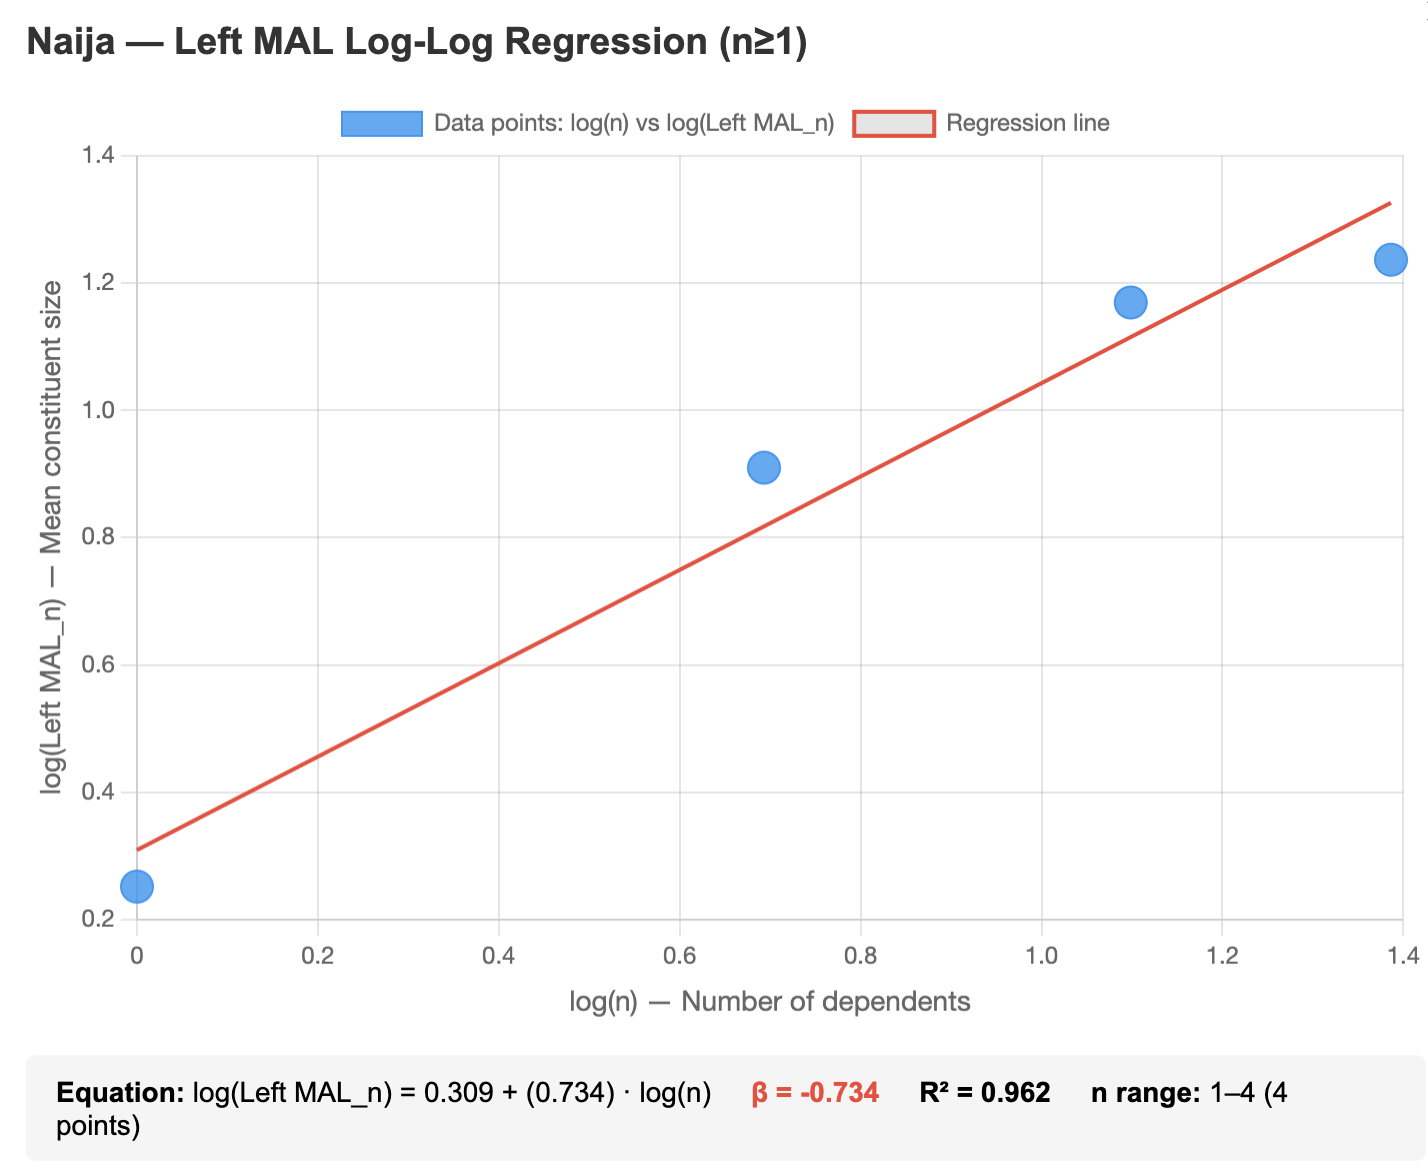
\includegraphics[width=\columnwidth]{latex/Naija-L.png}
\caption{$\lambda$MAL(Naija).}
\label{fig:Naija-L}
\end{center}
\end{figure}

\begin{figure}[!ht]
\begin{center}
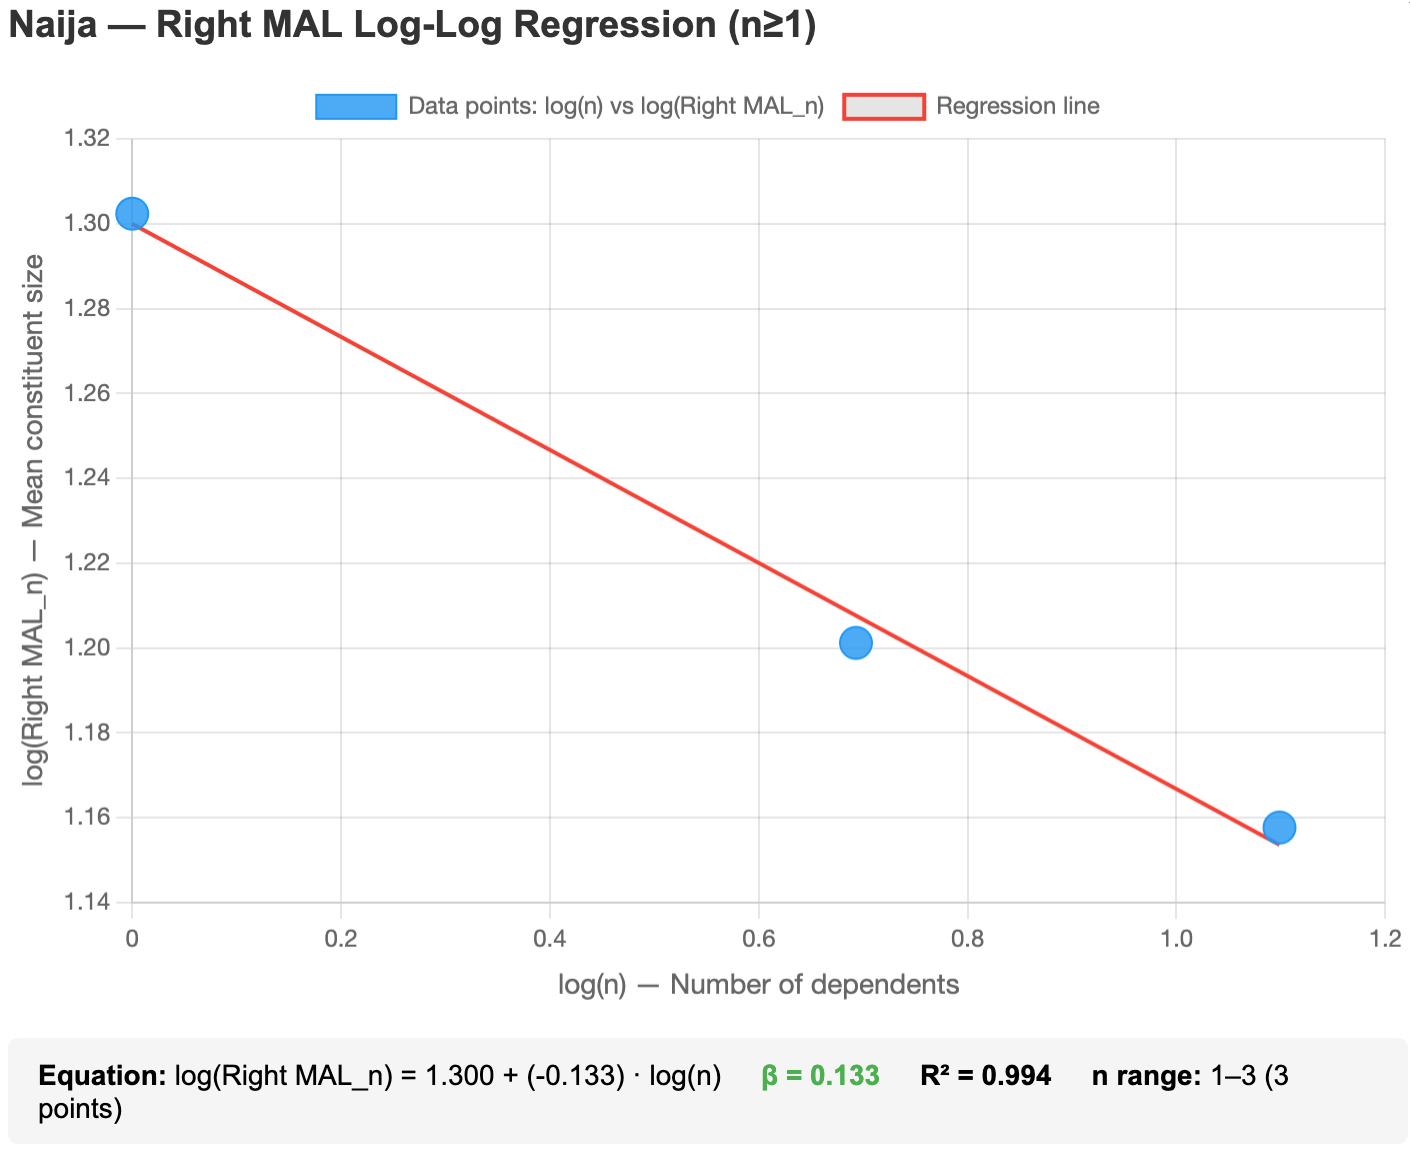
\includegraphics[width=\columnwidth]{latex/Naija-R.png}
\caption{$\lambda$MAL(Naija).}
\label{fig:Naija-R}
\end{center}
\end{figure}


As for the postverdal domain, we find the follwoing 7 Anti RMAL languages: Khoekhoe, Bambara, Egyptian, OldEastSlavic, WestArmenian, Gothic, and Latin. It is worth noting that among them, 4 are corpora of ancient languages:  Egyptian, OldEastSlavic, Gothic, and Latin. There are only 3 languages which are both Anti LMAL and Anti RMAL: Bambara, OldEastSlavic, and Latin. 

Exploring (gentic and/or areal) similarties and differences of these indiviual languages is beyond the scope of this paper, while it constitues a necessary avenue for future research in understanding length-based effects accross languages and linguistic domains.